\justifying 
System design provides the understanding and procedural details necessary for implementing
the system.Design builds coherent, well planned representations of programs that concentrate
on the interrelationships of parts at the higher level and the logical operations involved at the
lower levels. Software design is the first of the three technical activities designs, coding and test
which are required to build and verify the software

The organization of the Chapter is as follows.Section 4.1 describes the system architecture of the Virtual Lab Assistant. The Data Flow Diagrams (DFDs)
of the project are presented in Section 4.2. Section 4.3 covers various UML diagrams
including Use Case Diagram, Sequence Diagram, Collaboration Diagram, Class Dia-
gram, Component Diagram, and Deployment Diagram, the summary of the
chapter is provided in Section 4.4.

\section{System Architecture}
System architecture refers to the high-level design and structure of a complex system, outlining
its components, interactions, and organization to achieve specific objectives. It defines the
system’s key building blocks, functions, and how they communicate with each other and
external entities. A well-defined system architecture provides a blueprint for system
development, enabling efficient implementation, scalability, and maintenance while ensuring
that the system meets its intended goals and requirements. It often includes various
architectural layers, modules, interfaces, and data flows, which collectively shape the system’s
behavior and performance.

\begin{figure}[H]
    %\begin{center}
    \centering
    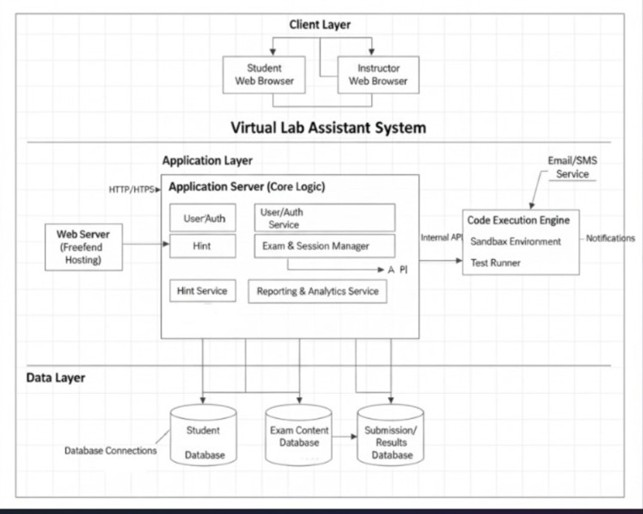
\includegraphics[width=15cm, height=12cm]{chapters/sysarchi.jpg}
    \caption{System Architecture}
    
    %\vspace{-0.3cm}
\end{figure}


\section{Data Flow Diagram}
A Data Flow Diagram (DFD) is a graphical representation used in system analysis and design to illustrate the flow of data within a system. It visually depicts processes, data stores, data flows, and external entities, providing a clear and concise overview of how data moves through a system and how different components interact. DFDs are instrumental in understanding, designing, and documenting information systems and processes.


\subsection{Level 0 DFD}
Level 0 Data Flow Diagram (DFD) is highest-level view of system’s data flow. It provides a simplified, bird’s-eye perspective, showing major processes or functions within system, external entities interacting with it, and primary data flows between them. Diagram serves as an initial overview of system architecture and helps stakeholders grasp system scope and boundaries.The Figure 4.2 shows Level 0 DFD Diagram.
\begin{figure}[H]
    %\begin{center}
    \centering
    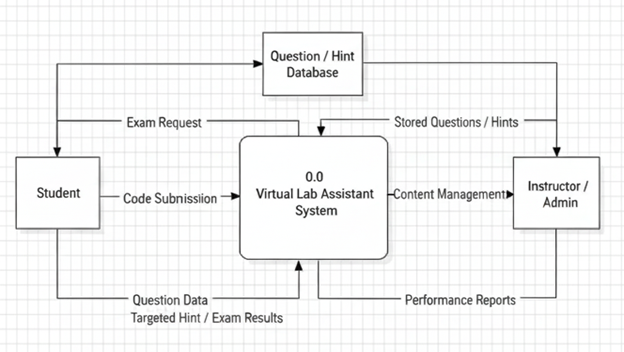
\includegraphics[width=15cm, height=5cm]{chapters/odfd.png}
 \caption{Level 0 DFD Diagram}\label{Fig:my_label}
    %\vspace{-0.3cm}

  \end{figure}
\subsection{Level 1 DFD}
A Level 1 Data Flow Diagram (DFD) is a more detailed representation that expands on the processes identified in the Level 0 DFD. It breaks down these processes into sub-processes or functions and provides a closer look at how data flows between them. Level 1 DFDs are used to gain a deeper understanding of the system's internal operations and data transformations, making them valuable for system analysis, design, and documentation. The Figure 4.3 shows Level 1 DFD Diagram.
\begin{figure}[H]
    %\begin{center}
    \centering
    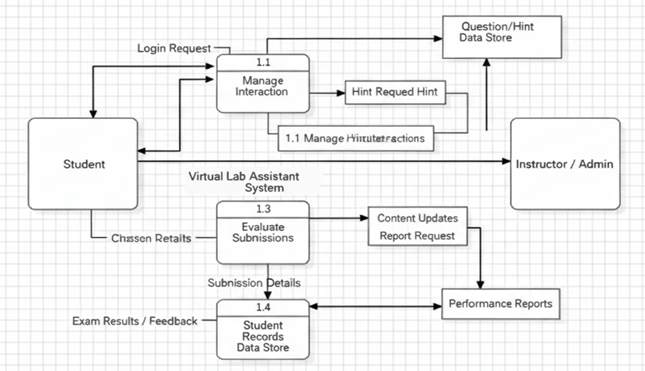
\includegraphics[width=15cm, height=8cm]{chapters/1dfd.png}
    \caption{Level 1 DFD Diagram}\label{Fig:my_label}
      
      \centering
\end{figure}


         \newpage  
\subsection{Level 2 DFD}
A Level 2 DFD is a detailed breakdown of processes from a Level 1 DFD, showing specific sub-processes, finer data flows, and detailed interactions with data stores and entities. It provides a deeper insight into how data is processed and managed within critical system components, aiding in precise system analysis and design. The Figure 4.4 shows Level 2 DFD Diagram
\begin{figure}[H]
    %\begin{center}
    \centering
    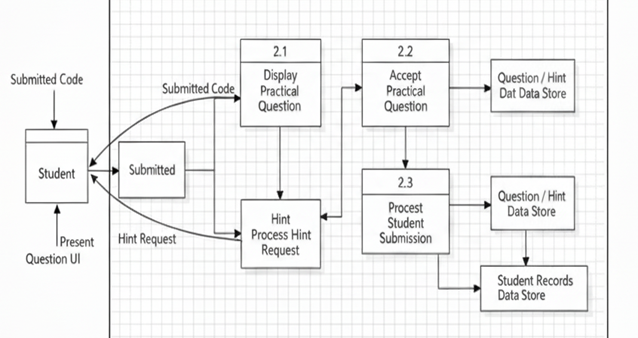
\includegraphics[width=15cm, height=12cm]{chapters/2dfd.png}
  \caption{Level 2 DFD Diagram}\label{Fig:my_label}
    %\vspace{-0.3cm}
\end{figure}

\newpage

\section{UML Diagrams}
Unified Modeling Language (UML) diagrams are a standardized set of visual representations used in software engineering and system design to model, document, and communicate complex systems and their components. UML diagrams include various types, such as Use Case diagrams for capturing system interactions, Class diagrams for depicting the structure and relationships of system objects, Sequence diagrams to show the sequence of interactions, Collaboration diagrams for illustrating collaborations among objects, and many more. These diagrams serve as powerful tools for software developers, designers, and stakeholders to visualize, analyze, and communicate the architecture, behavior, and interactions of software systems, enhancing the understanding and effectiveness of the design and development processes.



\subsection{Use Case Diagram}

Use case diagram shows the interaction between Use case which represents system functionality and actor which represent the people or system.The Figure 4.5 shows Use Case Diagram.

\begin{figure}[H]
    %\begin{center}
    \centering
    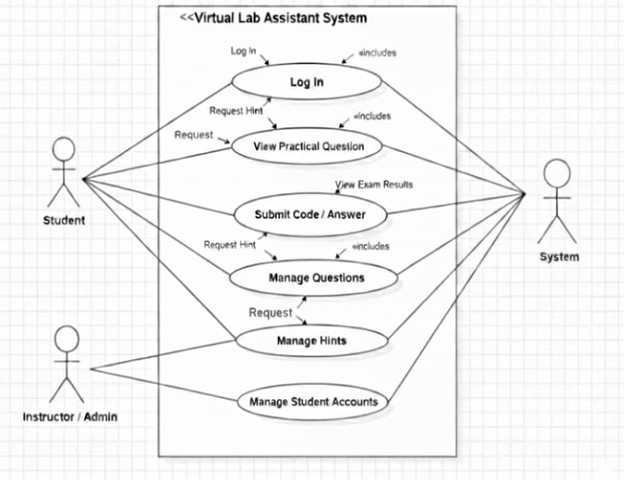
\includegraphics[width=13cm, height=15cm]{chapters/usecase.jpg}
    \caption{Use Case Diagram}\label{Fig:my_label}
    %\vspace{-0.3cm}
\end{figure}
\newpage

\subsection{Sequence Diagram}
The sequence diagram shows the flow of functionality through UseCase.A sequence diagram is a type of interaction diagram because it describes how and in what order a group of objects works together.These diagrams are used by software developers and business professionals to understand requirements for a new system or to document an existing process.The Figure 4.6 shows Sequence Diagram.


\begin{figure}[H]
    %\begin{center}
    \centering
    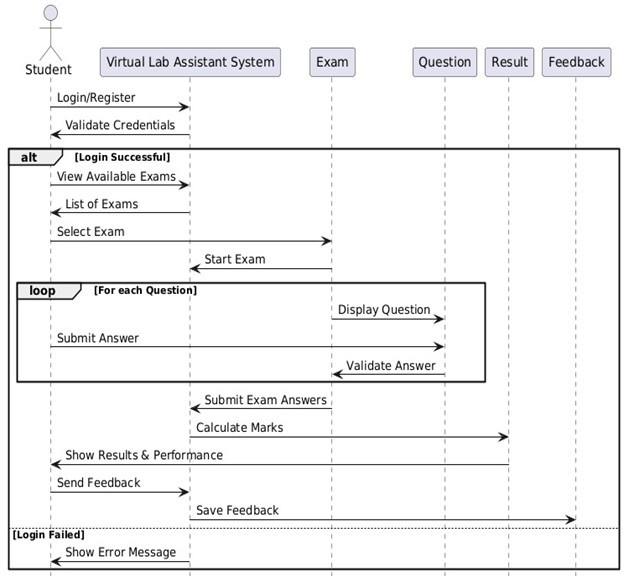
\includegraphics[width=15cm, height=13cm]{chapters/seq.jpg}
    \caption{Sequence Diagram }\label{Fig:my_label}
   % \caption{Sequence Diagram for Ideal Diet UseCase of Diet Planner Using BMI Calculation}
    %\vspace{-0.3cm}
\end{figure}
  % Figure :Sequence diagram for Admission Confirm use case of CAMS. 
\newpage




\subsection{Class Diagram}
The class diagram is the main building block of object- oriented modeling.It is used for general conceptual modeling of the structure of the application, and for detailed modeling translating the models into programming code.Class diagrams can also be used for data modeling.The Figure 4.7 shows Class Diagram.
\vspace{2cm}


\begin{figure}[H]
    %\begin{center}
    \centering
    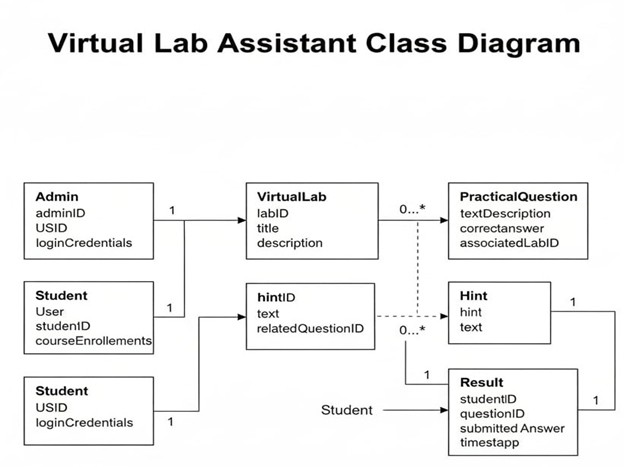
\includegraphics[width=15cm]{chapters/classi.jpg}
     \caption{Class Diagram}\label{Fig:my_label}
  %  \caption{Class Diagram for Diet Planner using BMI calculation}
    %\vspace{-0.3cm}
\end{figure}
\newpage




\subsection{Component Diagram}
A component diagram, also known as a UML component diagram, describes the organization and wiring of the physical components in a system.Component diagrams are often drawn to help model implementation details and double check that every aspect of the system’s required functions covered by planned development.The Figure 4.8 shows Component Diagram.


\begin{figure}[H]
    %\begin{center}
    \centering
    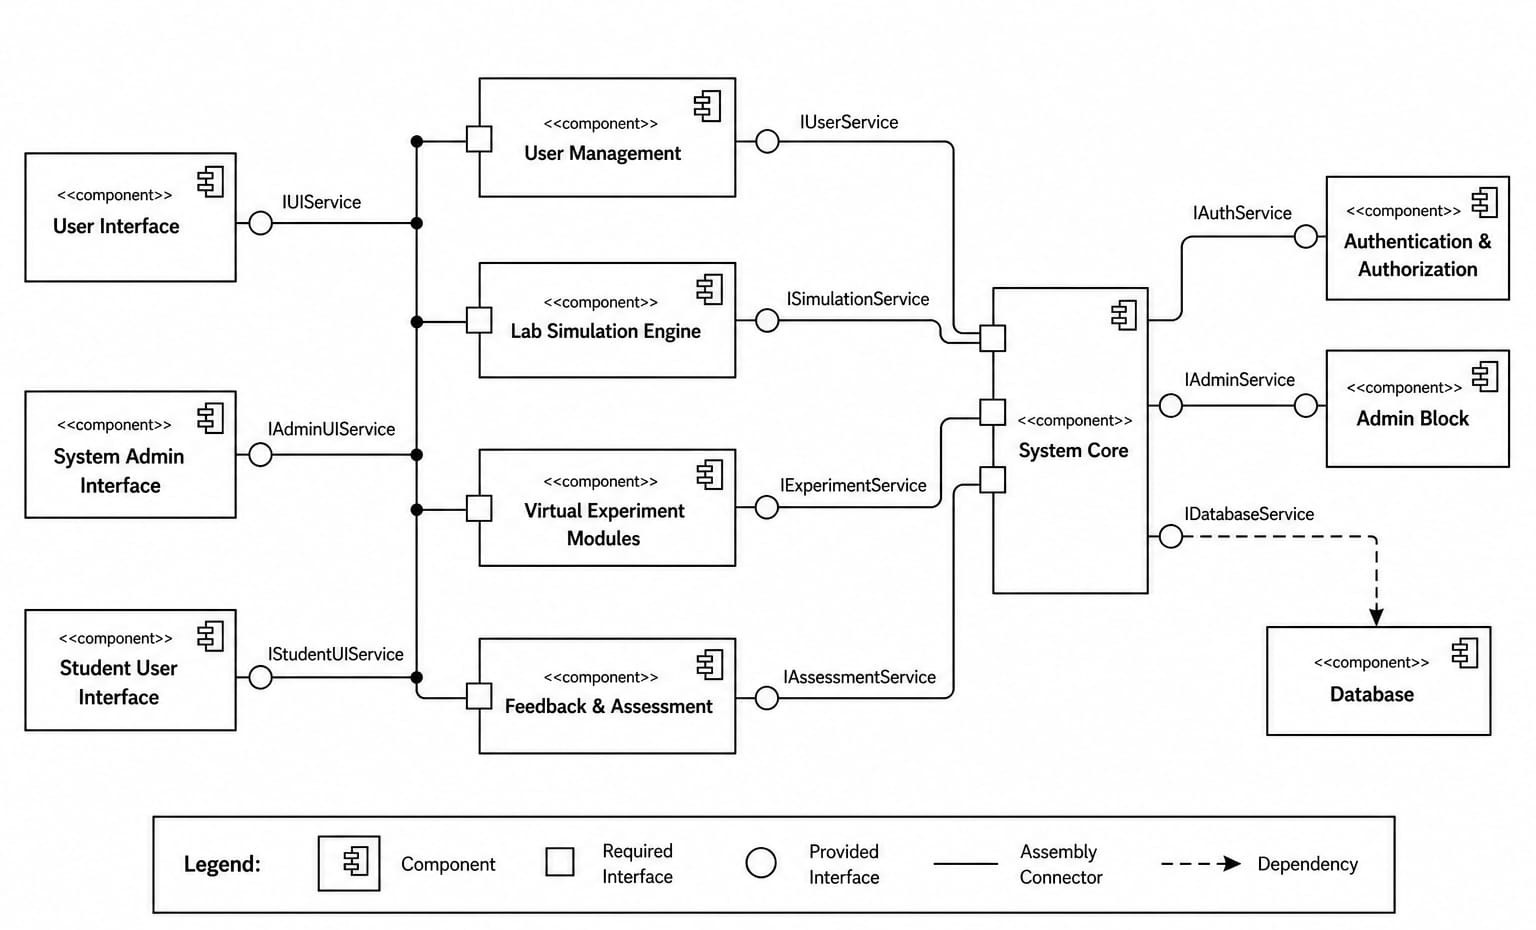
\includegraphics[width=15cm]{chapters/compo.jpeg}
      \caption{Component Diagram}\label{Fig:my_label}
   % \caption{Component Diagram For Diet Planner using BMI Calculation}
    %\vspace{-0.3cm}
\end{figure}
\newpage

\subsection{Deployment Diagram}
A deployment diagram is a UML diagram type that shows the execution architecture of a system, including nodes such as hardware or software execution environments, and the middle ware connecting them.Deployment diagrams are typically used to visualize the physical hardware and software of a system.The Figure 4.9 shows Deployment Diagram.


\begin{figure}[H]
    %\begin{center}
    \centering
    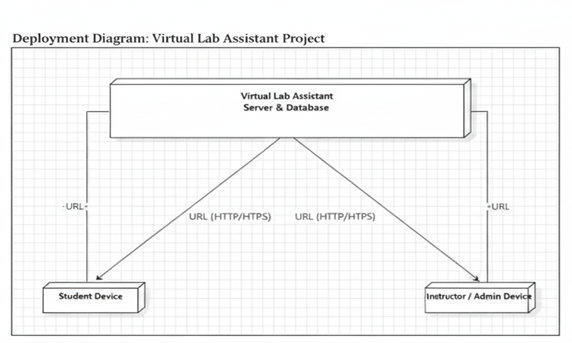
\includegraphics[width=15cm]{chapters/dep.png}
    \caption{Deployment Diagram}\label{Fig:my_label}
   % \caption{Deployment Diagram for Diet Planner using BMI Calculation}
    %\vspace{-0.3cm}
\end{figure}
\section{Summary}
n this Chapter, Design is presented. In the next Chapter, the Coding and Implementation
will be discussed .


